%IMD PNA http://na.support.keysight.com/pna/help/latest/Applications/Swept_IMD_Configure_External_Source_and_Combiner.htm
\chapter{Desarrollo}



%%-----------------------------------------------------------------------

\section{Desarrollo del proyecto}

\subsection{Datos}

La base de datos de archivos midi que se utilizo en este proyecto se llama ''Clean MIDI subset'' la cual se uso en el proyecto \cite{Lear_Coli}. Esta base de datos contiene m�s de 17,000 canciones en formato MIDI, estas canciones son en su mayor�a del g�nero Pop y Rock, por lo que la red utilizada en este proyecto fue entrenada para asimilar este tipo de estilos.

Para el procesamiento de los archivos MIDI se utilizo una librer�a de software libre llamada Music21, la cual nos permite de una manera f�cil trabajar con estos archivos. Esta librer�a es compatible con Python3 por lo que nuestro programa esta hecho en este lenguaje de programaci�n.

\subsubsection{Delimitaci�n de los Datos}

Esta es una base de datos demasiada extensa por lo que el tiempo de procesamiento puede ser excesivo si se introducen los datos directamente a una red neuronal, debido a esto se decidi� dividirla y solamente usar una parte de ella (1000 canciones unicamente).

Cada canci�n tiene una duraci�n promedio de 3 minutos por lo que aunque se este usando solo una parte de las canciones la cantidad de datos es suficiente para lograr entrenar la red con buenos resultados.

Los archivos MIDI de esta base de datos poseen diferentes Tracks de varios instrumentos de los cuales en este proyecto solamente se tomaran en cuenta los Tracks de guitarra el�ctrica limpia, bajo el�ctrico con dedos y bater�a, los demas Tracks ser�n ignorados.

\subsection{Descripci�n del proyecto}

\subsubsection{Red Neuronal} 

La intensi�n de este proyecto es crear una serie de redes neuronales que sean capaces de procesar las entradas de guitarra, bajo y bateria, Para esto se usaron 3 redes neuronales por separado para procesar los instrumentos, estas redes tienen la siguiente arquitectura:

\begin{figure}[htbp]
	\centerline{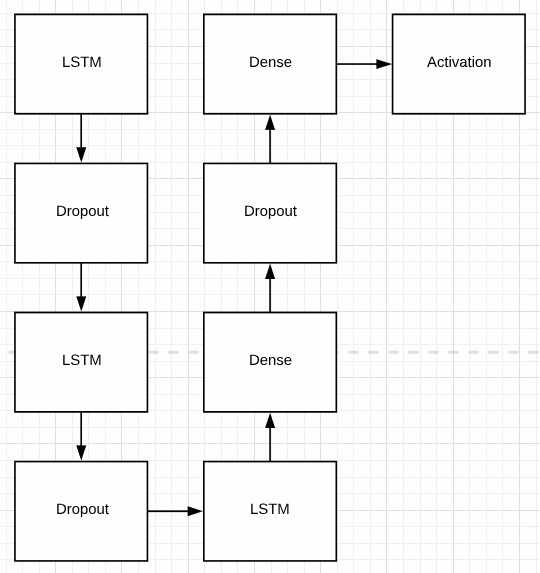
\includegraphics[width=8cm]{estruc_red.png}}
	\caption{Estructura de la Red neuronal}
	\label{fig:estruc_red}
\end{figure}

Las capas de redes LSTM procesan de manera secuencial la informaci�n de las matrices generadas a partir de los eventos en los Tracks, las capas de Dropout son usadas para prevenir el sobre entrenamiento de la red, eliminando algunos datos de salida de las redes LSTM, finalmente llega a una capa Dense la cual nos ayuda al aprendizaje de la red. 

La funci�n de activaci�n que se uso en esta red es una $tanh$, este tipo de activaci�n permite de una manera mas suavizada la activaci�n o desactivaci�n de las neuronas en comparaci�n con una se�al sigmoidea

\subsubsection{Arquitectura de la aplicaci�n}

La arquitectura de la aplicaci�n se muestra en la siguiente figura:

\begin{figure}[htbp]
	\centerline{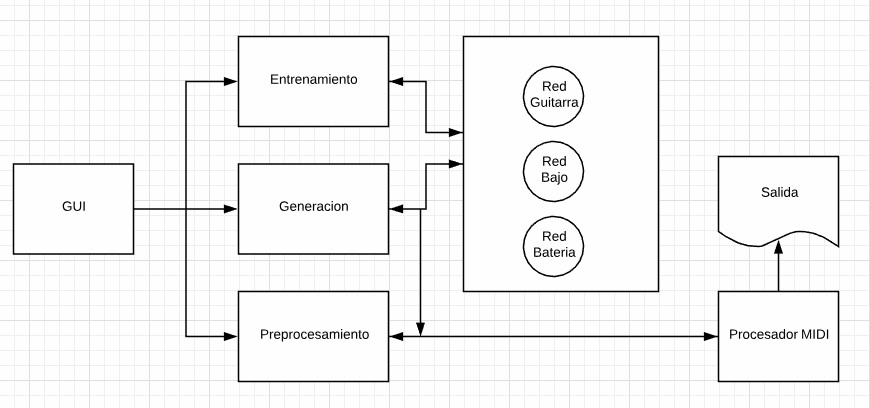
\includegraphics[width=10cm]{arq_app.png}}
	\caption{Arquitectura de la aplicaci�n}
	\label{fig:arq_app}
\end{figure}

En esta arquitectura se puede observar que se tiene varios m�dulos el sistema:

\begin{enumerate}
	\item \textbf{GUI.-} Este modulo contiene la interfaz de usuario para el programa.
	\item \textbf{Preprocesamiento.-} Este modulo se encarga de preprocesar los archivos MIDI con el fin de separar los tracks de guitarra, bajo y bater�a en diferentes archivos MIDI.
	\item \textbf{Entrenamiento.-} Este modulo se encarga de entrenar la red con los archivos MIDI previamente preprocesados.
	\item \textbf{Generaci�n.-} Este modulo genera nuevas piezas a partir de enviar notas al azar a la red entrenada.
	\item \textbf{Redes neuronales.-} En este modulo se tienen 3 redes neuronales completamente independientes, una para guitarra, otra para bajo y la ultima para bater�a.   
	\item \textbf{Procesador MIDI.-} Este modulo contiene todas las utiler�as para el manejo de los archivos MIDI.
\end{enumerate}

\subsection{Proceso de entrenamiento}

%TODO: documentar todo el proceso de entrenamiento y los resultados
\subsection{Validaci�n de resultados}

%TODO: documentar los resultados y el proceso de su validaci�n